%% This is emulateapj reformatting of the AASTEX sample document
%%
\documentclass[iop]{emulateapj}

\newcommand{\vdag}{(v)^\dagger}
\newcommand{\myemail}{skywalker@galaxy.far.far.away}

%% You can insert a short comment on the title page using the command below.

\slugcomment{Not to appear in Nonlearned J., 45.}

%% If you wish, you may supply running head information, although
%% this information may be modified by the editorial offices.
%% The left head contains a list of authors,
%% usually a maximum of three (otherwise use et al.).  The right
%% head is a modified title of up to roughly 44 characters.
%% Running heads will not print in the manuscript style.

\shorttitle{Size - Star Formation}
\shortauthors{Phillips et al.}

%% This is the end of the preamble.  Indicate the beginning of the
%% paper itself with \begin{document}.

\begin{document}

%% LaTeX will automatically break titles if they run longer than
%% one line. However, you may use \\ to force a line break if
%% you desire.

\title{The Relationship Between Size and Star Formation in Active Galaxies}

%% Use \author, \affil, and the \and command to format
%% author and affiliation information.
%% Note that \email has replaced the old \authoremail command
%% from AASTeX v4.0. You can use \email to mark an email address
%% anywhere in the paper, not just in the front matter.
%% As in the title, use \\ to force line breaks.

\author{J. I. Phillips\altaffilmark{1,2,3} and Claudia Scarlata \altaffilmark{1}}
\affil{Minnesota Institute for Astrophysics, University of Minnesota,
    Minneapolis, MN 55455}

%% Notice that each of these authors has alternate affiliations, which
%% are identified by the \altaffilmark after each name.  Specify alternate
%% affiliation information with \altaffiltext, with one command per each
%% affiliation.


%% Mark off your abstract in the ``abstract'' environment. In the manuscript
%% style, abstract will output a Received/Accepted line after the
%% title and affiliation information. No date will appear since the author
%% does not have this information. The dates will be filled in by the
%% editorial office after submission.

\begin{abstract}
We examine a sample of SDSS galaxies with masses between $10^{8.5}$ and $10^{10.5}$ for signatures of radial feedback driven by bursty star formation. We measure each galaxy's offset from the median size-mass relation, and plot this excess size against their $H\alpha$ emission. Below $10^{9.5}$, we see a negative correlation between galaxy size and $H\alpha$ emission, i.e., actively star-forming galaxies are more compact. This is strong observational evidence for a ``breathing'' mode of star formation, where intense star formation in the galactic center drives radial outflows of gas and stars in a cyclic fashion. More massive galaxies do not show the same correlations between size and star formation activity, consistent with the observations that these objects reside in cuspy dark matter halos. Additionally, we examine the radial profile of star formation in both dwarf and massive galaxies, finding star formation far more concentrated in dwarf galaxies.
\end{abstract}

%% Keywords should appear after the \end{abstract} command. The uncommented
%% example has been keyed in ApJ style. See the instructions to authors
%% for the journal to which you are submitting your paper to determine
%% what keyword punctuation is appropriate.

%% Authors who wish to have the most important objects in their paper
%% linked in the electronic edition to a data center may do so in the
%% subject header.  Objects should be in the appropriate "individual"
%% headers (e.g. quasars: individual, stars: individual, etc.) with the
%% additional provision that the total number of headers, including each
%% individual object, not exceed six.  The \objectname{} macro, and its
%% alias \object{}, is used to mark each object.  The macro takes the object
%% name as its primary argument.  This name will appear in the paper
%% and serve as the link's anchor in the electronic edition if the name
%% is recognized by the data centers.  The macro also takes an optional
%% argument in parentheses in cases where the data center identification
%% differs from what is to be printed in the paper.

%\keywords{globular clusters: general ---
%globular clusters: individual(\objectname{NGC 6397},
%\object{NGC 6624}, \objectname[M 15]{NGC 7078},
%\object[Cl 1938-341]{Terzan 8})}

%% From the front matter, we move on to the body of the paper.
%% In the first two sections, notice the use of the natbib \citep
%% and \citet commands to identify citations.  The citations are
%% tied to the reference list via symbolic KEYs. The KEY corresponds
%% to the KEY in the \bibitem in the reference list below. We have
%% chosen the first three characters of the first author's name plus
%% the last two numeral of the year of publication as our KEY for
%% each reference.

\section{Introduction}
\label{intro}

Dwarf galaxies, galaxies at or below stellar mass of $\sim 10^{9.5} M_{\odot}$, are important laboratories that allow us to study structure formation at the smallest scales. In particular, their ratios of baryons to dark matter are extremely low, typically around 1:100. This gives rise to important differences in the structure and star formation histories of dwarf galaxies as compared to more massive galaxies, and studying these differences can shed light on important physics related to how galaxy formation is regulated by both baryons and dark matter.

Cosmological simulations based on the preferred cold dark matter model ($\Lambda$CDM) predict that galaxies form in self-similar halos of dark matter, which have density profiles described by a double power law with an inner logarithmic slope of -1, termed a Navarro-Frank-White (NFW) profile \citep{NFW}. The distribution statistics and kinematics of massive galaxies is fully consistent with them living in dark matter halos with NFW profiles \citep{Wambsganss04,Springel05,BK09,Klypin11}; however, dwarf galaxy kinematics are better described by halos with a flat inner slope, typically referred to as a ``cored'' profile \citep{Moore94,McGaugh01,Marchesini02,Simon05,deblok08}. This tension between predictions made from $\Lambda CDM$ and observations is termed the ``core-cusp problem.'' A closely related problem, the ``too big to fail problem,''  notes that satellite halos (or subhalos) seen around Milky-Way-like galaxies in $\Lambda$CDM simulations are too dense to host any of the observed Milky Way dwarf satellites \citep{BK11,BK12}. Note that these two problems may indeed be two manifestations of the same problem, i.e., both problems may be solved if halos in the real Universe have cored profiles. Recent work by \cite{GK14} demonstrated that the ``too big to fail'' problem extended beyond the Milky Way's virial radius, suggesting that the problem has more to do with how dwarf galaxies form than how environmental effects such as ram-pressure stripping or tidal interactions manifest (See, e.g., \citet{Gunn72,Larson80,Farouki81,Moore96,Balogh2000} for a discussion of these effects).

In order to resolve these problems, one of two things must be true. Either the underlying physics of $\Lambda$CDM must be modified in some way, or baryonic processes must be invoked to bridge the gap between theory and observation. Recent work has been dedicated to exploring both possibilities. On the cosmological side, both self-interacting dark matter and warm dark matter can serve to suppress structure formation and lower the central densities of dark matter halos \citep{Lovell14,Elbert14}. With respect to baryonic matter, supernova feedback has long been known to deposit energy into the interstellar medium (ISM), driving galactic winds \citep{Larson74,Dekel86}. More recently, this feedback has been posited as a mechanism by which energy may be injected into dark matter particles, kinematically warming them. Several authors have argued that if star formation proceeds in bursts in dwarf galaxies, energy will be injected with enough efficiency to create cores in the centers of dark matter halos \citep{Governato10,Governato12,PG12}. Observational studies have demonstrated that, for dwarf galaxies in particular, the star formation rate as measured by $H\alpha$ has more scatter than the star formation rate as measured by FUV emission \citep{Sullivan00,Boselli09,Lee09,Shivaei15,Guo16,Sparre17}. Since these indicators trace star formation over different timescales, these studies are consistent with a picture where star formation in dwarfs is stochastically bursty; however, radial transport driven by this stochastic star formation remains unobserved.

One clue to resolving this dilemma may lie in how dwarf galaxies' old stars are distributed. While exceptions abound, massive galaxies generally have concentrations of old stars in the center, and younger stars in the outskirts \citep{dejong96,Bakos08}. Dwarf galaxies, on the other hand, typically show the inverse; young stars in the center and old stars on the outskirts \citep{Hidalgo09,Hidalgo13}. Several studies have argued that these radial age gradients arise from in situ formation; old stars in the external region were born there at early times and generally remained there, exhibiting only minor radial movement with no preferred direction \citep{Stinson09,Schroyen13}. However, recent simulations have raised the possibility that stars in dwarf galaxies experience significant radial transport; young stars are born in galactic interiors, then at some point in their lifetimes they move to larger radii, possibly driven by feedback \citep{Gonz16,EB17}. Distinguishing between these two possibilities could shed light on the physics behind dwarf galaxy formation.

A unified model of galaxy formation that solves these problems was first put forward by \cite{Navarro96}, where the authors show that feedback driven outflows can produce galaxies in simulations with realistically cored profiles. Further studies \citep{Governato10,Governato12,Maxwell12,DC14,Pontzen14,Chan15,EB17} refined the theory, specifying that feedback regulates dwarf galaxy star formation in a stochastic manner and powers radial transport, but an observational smoking gun for this model remains elusive. 

In this study, we use observations of both dwarf galaxies and massive galaxies to investigate the observational predictions of a model for dwarf galaxy formation whereby stochastic star formation in the center of the galaxy powers radial transport of both baryonic and dark matter. Specifically, our study will focus on the structure of star forming galaxies, and how that structure is dependent on the vigor with which the galaxy is forming stars. [Description of sections]. Throughout the paper we use h=0.7 in appropriate calculations, [other relevant details]. 

\section{Data and observations}
\label{sec:obs}

The data used in this study come from the Sloan Digital Sky Survey \citep[SDSS,][]{SDSS}, making use of the NYU and MPA-JHU value-added galactic catalogs \citep{Kauffmann03,Brinchmann04,blanton05vagc}. To select our scientific sample, we first select all galaxies with stellar masses between $10^{8.5}$ and $10^{10.5} M_{\odot}$. We require galaxies in our scientific sample to be actively star forming, so we impose a minimum $H\alpha$ equivalent width of $2 \rm \AA$ and require that the galaxies we select reside in the purely star forming region of the BPT diagram \citep{BPT}. We admit to the scientific sample only galaxies within a mass-dependent completeness redshift, estimated by dividing the sample into four mass bins of width 0.5 dex and plotting a histogram of the redshift of galaxies in each bin. The peak of the histogram was taken to be the approximate completeness limit for the scientific sample. These limits, as well as the number of galaxies in our sample, are given in Table \ref{tab:info}.

%We also put together a sample that would be used to calibrate our required fiber corrections. This sample was selected in exactly the same way as the scientific sample, except the completeness requirement was relaxed; galaxies were permitted into the calibration sample if they were within two times the completeness limit of the scientific sample. In \ref{sec:fibercor}, we describe how this calibration sample is used.

\subsection{Central star formation}
\label{sec:fibercor}
SDSS spectroscopy is based on light being channeled into fibers $3$ arcsec in diameter. This gives us an opportunity to more closely probe the star formation rate in the galaxy's central regions. Since we will be interested in star formation happening in the galaxy's center, we will define a fiber-corrected star formation rate that intentionally overly relies on measurements at the galaxy center, which we will call $\rm SFR_{cent}$. Eventually, we will be interested in whether or not $\rm SFR_{cent}$ is larger or smaller than the galaxy's true star formation rate, which will give us a measure of how centrally concentrated the star formation is, but first we will detail how $\rm SFR_{cent}$ is calculated.

We begin by defining a parameter $\Psi$ that corresponds to the fraction of a galaxy's area on the sky that lies within the fiber. For galaxies smaller than 3 arcsec, $\Psi = 1$. For larger galaxies, $\Psi = \frac{\pi R^2}{A_z}$, where R is the circularized radius of the galaxy measured in kpc (taken to be \textit{r}-band R90 so as to account for nearly all light from the galaxy) and $A_z$ is the area of a circle of diameter 3 arcsec at the redshift of the galaxy. Figure \ref{fig:geo} shows $\Psi$ plotted against galaxy radius for galaxies in our $10^{9.5}-10^{10.0}$ bin. Notice that, as one might expect, larger galaxies tend to have more of their area fall outside out the fiber, leading to lower values of $\Psi$. The selection effect in the upper right portion of the plot is introduced by the redshift cut we place on the sample. An object that lies on this line is located close to the maximum allowed redshift, such that it is the minimum size on the sky, and thus the largest $\Psi$. 

If we are carrying out a correction on some generic parameter $\Theta$, which could represent e.g. star formation rate, we assume that the correction will take the form of a power law, i.e., $$\Theta_{total} = \Theta_{fiber} \times \Psi^{-\alpha}$$. Here $\alpha$ is a power law index that we will derive empirically and $\Theta_{fiber}$ is the measured value of $\Theta$ within the fiber. In calculating $\alpha$, our goal is to correct $\Theta$ such that it its distribution independent of redshift (we assume no redshift evolution within our full sample). To this end, we fit a linear relationship to $log \Theta_{fiber}$ and $log \Psi$. The slope of this relationship we adopt as $\alpha$.

To validate that our correction procedure does indeed produce a measure for $\Theta$ that is independent of redshift, we divide each mass bin on redshift. We will refer to these as the low redshift subsample and high redshift subsample\footnote{We use "high" redshift in a relative sense; all galaxies we consider in this paper are quite low redshift.}. Galaxies with redshift less than $z_{complete}/2$ are placed in the low redshift subsample, and with redshifts between $z_{complete}/2$ and  $z_{complete}$ in the high redshift sample. In applying the correction, we will call the measured value of the parameter of interest $\Theta_{fiber}$. We then compare at the distributions in $\Theta_{total}$ between the low and high redshift sample. This comparison is shown in $H_\alpha$ luminosity in Figure \ref{fig:hist} for the $M\star ~ 10^{9.5} M_{\odot}$ bin. We see excellent agreement in the corrected values across redshift for each mass bin, and note that this agreement is only seen after the correction is made. Table \ref{tab} contains the measured alphas and completeness redshifts for each sample. If we substitute $SFR$ for the generic $\Theta$ in the above derivation, we can make explicit the definition $$SFR_{cent} \equiv SRFR_{fiber} \times \Psi^{-alpha}$$.

\subsection{Concentration/luminosity degeneracy}
\label{sec:concdep}
As previously mentioned, the above procedure produces a measure for $SFR_{cent}$ that is overly reliant on information from the galaxy's center. If two galaxies have the same $\Psi$ and $SFR_{fiber}$, they would end up with the same $SFR_{cent}$, even if one of them had substantially more star formation in its outskirts (and thus a higher true star formation rate). Essentially, using the parameter $SFR_{cent}$ introduces a degeneracy between a galaxy's true star formation rate and the concentration of its star formation. Note that, had we simply corrected for the area outside of the fiber (i.e., applied an $\alpha= 1$ correction), we would have been degenerate in redshift as well.

To investigate this degeneracy, we carried out a simple Monte Carlo simulation with toy models of galaxies. The galaxies displayed star formation according to one of three models: they either have centrally concentrated star formation, constant star formation density, or star formation preferentially in the outskirts. Galaxy size and overall star formation rate was allowed to vary. We then applied the same steps described above to determine a $SFR_{cent}$ for our simulated galaxies. Upon plotting $SFR_{cent}$ vs. $\Psi$, the three models occupy distinct regions of parameter space, with the objects with centrally concentrated star formation displaying the highest $SRF_{cent}$ and the objects with low central star formation displaying the lowest. To remove the variation due to intrinsic star formation, we normalize $SFR_{cent}$ by each galaxy's intrinsic star formation rate. This allows us to examine $\rm log \frac{SRF_cent}{SFR}$ for each galaxy as the ``central excess" in star formation. If we color the points in $\rm log \frac{SRF_cent}{SFR}$ vs. $\Psi$ space by concentration (i.e., R90/R50) we can see a correspondence between high $\rm log \frac{SRF_cent}{SFR}$ and concentration. We will therefore use this ratio as a proxy for the concentration of star formation in our galaxies. 

%%%%%%%%%%%%%%%%%%%%%%%%%%%%%%%%%%%%%%%%%%%%%%%%%%%%%%%%%%%%%%
\begin{table}[]
	\centering

	\label{tab:info}
	\begin{tabular}{lll} 
	\hline 
	Mass Bin ($M_{\odot}$)& $\alpha$ & $z_{\rm complete}$ 	\\
	\hline
	\hline 
	$10^{8.5}$   & 0.835 & 0.023 \\ 
	$10^{9.0}$   & 0.740   & 0.035  \\ 
	$10^{9.5}$   & 0.784    & 0.058 \\ 
	$10^{10.}$   &  0.664 & 0.07 \\
	\hline 
	\end{tabular}
		\caption{Power law index and completeness redshift for galaxies in each mass bin we consider. }
\end{table}
%%%%%%%%%%%%%%%%%%%%%%%%%%%%%%%%%%%%%%%%%%%%%%%%%%%%%%%%%%%%%%


%%%%%%%%%%%%%%%%%%%%%%%%%%%%%%%%%%%%%%%%%%%%%%%%%%%%%%%%%%%%%%
\begin{figure*}
	\centering
	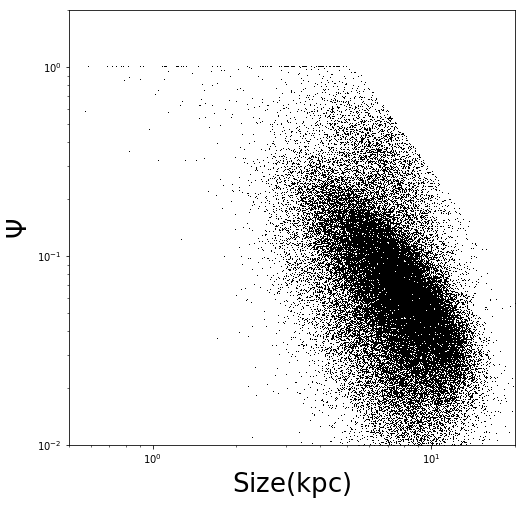
\includegraphics[width=1 \columnwidth]{geometry_9_5.png}
	\caption{Geometric parameter $\Psi$ plotted vs. physical size for galaxies in the $10^{10} - 10^{10.5} M_{\odot}$ mass bin. $\Psi$ measures the fraction of the galaxy that falls within the SDSS fiber. The selection effect arises due to the cut in redshift space.}
     \label{fig:geo}

\end{figure*}
%%%%%%%%%%%%%%%%%%%%%%%%%%%%%%%%%%%%%%%%%%%%%%%%%%%%%%%%%%%%%% 

%%%%%%%%%%%%%%%%%%%%%%%%%%%%%%%%%%%%%%%%%%%%%%%%%%%%%%%%%%%%%%
\begin{figure*}
	\centering
	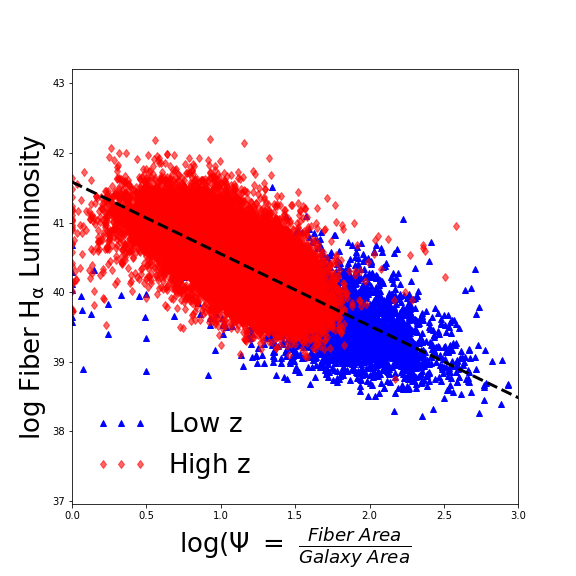
\includegraphics[width= \columnwidth]{alpha_regression_9_5.png}
	\caption{The relationship between the geometric factor $\Psi$ measuring the ratio of a galaxy's size to the size of the SDSS fiber and the fiber $H_{\alpha}$ luminosity for galaxies in the $10^{9.5} - 10^{10} M_{\odot}$ bin. Knowing the average functional form of this relationship allows us to correct for fiber effects. Points marked with a blue triangle are at lower redshift than those marked with a red diamond}
     \label{fig:steps}

\end{figure*}
%%%%%%%%%%%%%%%%%%%%%%%%%%%%%%%%%%%%%%%%%%%%%%%%%%%%%%%%%%%%%% 

%%%%%%%%%%%%%%%%%%%%%%%%%%%%%%%%%%%%%%%%%%%%%%%%%%%%%%%%%%%%%%
\begin{figure*}
	\centering
	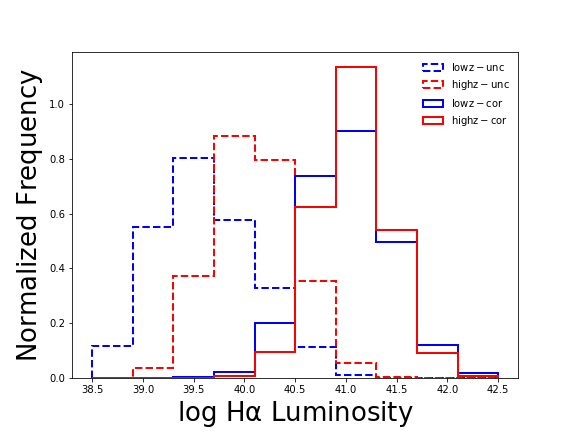
\includegraphics[width=1 \columnwidth]{Lum_hist_9_5.png}
	\caption{Histogram of $H\alpha$ luminosities for the uncorrected (dashed blue line) and corrected (solid blue line) low z calibration set, along with the uncorrected (dashed red line) and corrected (solid red line) high z calibration set. Correcting both sets brings them into agreement.}
     \label{fig:hist}

\end{figure*}
%%%%%%%%%%%%%%%%%%%%%%%%%%%%%%%%%%%%%%%%%%%%%%%%%%%%%%%%%%%%%% 

%%%%%%%%%%%%%%%%%%%%%%%%%%%%%%%%%%%%%%%%%%%%%%%%%%%%%%%%%%%%%%
\begin{figure*}
	\centering
	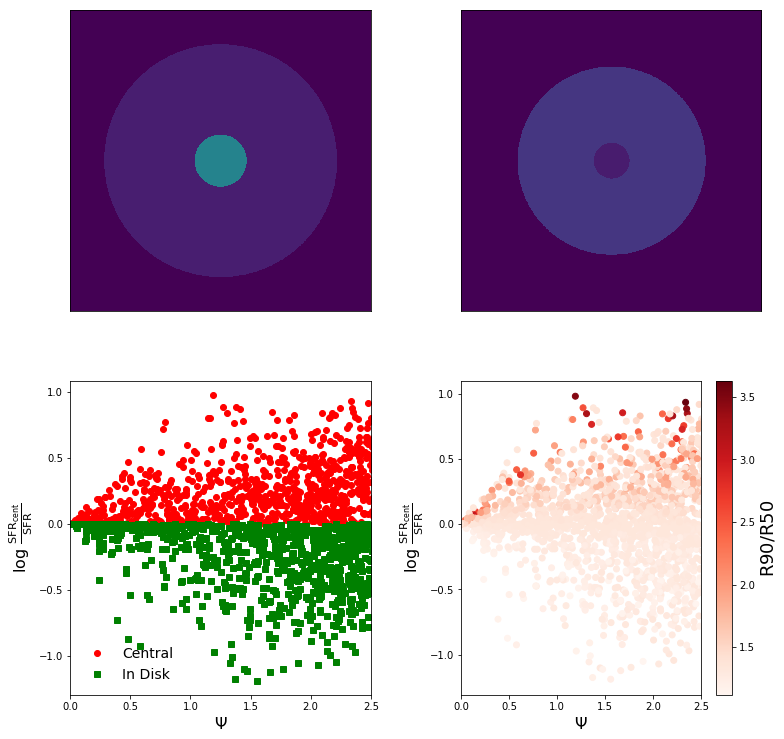
\includegraphics[width=1.4 \columnwidth]{model.png}
	\caption{\textit{Top:} Examples of allowed toy star-forming models; \textit{left}: centrally concentrated star formation, \textit{center}: constant star formation density, \textit{right}: star formation preferentially in the outskirts. \textit{Bottom:} $\rm log \  SFR_{cent}$ vs. $\Psi$ colored by (\textit{left}) model, and (\textit{right}) concentration.}
	\label{fig:model}
	
\end{figure*}
%%%%%%%%%%%%%%%%%%%%%%%%%%%%%%%%%%%%%%%%%%%%%%%%%%%%%%%%%%%%%% 


\section{Results}
\label{sec:results}

In this section we will examine the relationship between a galaxy's physical size and the rate and concentration of its star formation. Our sample is divided into bins of 0.5 dex in stellar mass, allowing us to examine how the relationship between size and $H\alpha$ emission with galaxy mass. Of particular interest is what happens at dwarf-scale masses, i.e., the lower two mass bins of our sample.

To establish a mass-independent size metric, we fit a mass-size relation to all star-forming galaxies below redshift 0.03, then determine the expected size for each galaxy in the sample based on its stellar mass. For each galaxy, we then calculate a ``size offset" which is the logarithm of the ratio between the actual size of the galaxy in kpc and the expected size of that galaxy, also in kpc. This size offset parameter has the useful properties of being centered at or very close to zero for any given population of galaxies, and having relatively consistent scatter (about 0.4 dex) over the mass ranges we probe.

%In Figure \ref{fig:HA_ew}, we plot the total (i.e. aperture-corrected) $H\alpha$ equivalent width against the size offset parameters in four stellar mass bins. There is an anti-correlation in $H \alpha$ equivalent width with galaxy size in all four bins, however  this anti-correlation is most significant in the lowest mass bin. To emphasize this point, we show the median equivalent width for galaxies with negative size offset (i.e. smaller size, black points) and positive size offset (i.e. larger size, green points) as horizontal lines. In Figure \ref{fig:HA_ew_mass}, we show the difference between these two medians plotted against stellar mass. Here, $\rm \Delta log(H_{\alpha}\ EW)$ is defined to be the median equivalent width of the larger galaxies minus that of the smaller galaxies. Here it is apparent that equivalent widths of the sample at $10^{8.5} \ M_{\odot}$ are significantly lower than those at higher masses.

In Figure \ref{fig:sfr}, we plot star formation rate against size offset for galaxies in each mass bin. As expected, star formation tends to increase with increasing mass. Within each mass bin, we plot the average star formation rate at fixed size offset as a blue line. In the lowest mass bin, the slope of average star formation rate is flat, i.e., larger galaxies are forming stars no more vigorously than their smaller counterparts. With increasing mass, the slope of the relation between size and star formation steepens, such that larger galaxies are indeed forming more stars. 

We compute the difference in the median star formation rate for objects that have larger and smaller than average for their mass. These galaxies are colored green and black, respectively, in Figure \ref{fig:sfr}. We plot this difference in Figure \ref{fig:HA_lum_mass}. Errors on the median values were determined through bootstrapping. Galaxies of mass $10^{8.5} M_{\odot}$ have the smallest difference in median star formation rate. More massive galaxies have larger differences, although the effect is not monotonic. Galaxies at $10^{9} M_{\odot}$ and $10^{10} M_{\odot}$ in stellar mass show roughly equal difference between small and large galaxies, and galaxies at $10^{9.5} M_{\odot}$ show the greatest difference.

It should be said that this effect is somewhat subtle. Even the largest discrepancy in star formation between small and large galaxies we observe results in only a $20\%$ boost in star formation for larger galaxies. On the other hand, the equivalence of star formation rate between large and small galaxies in the lowest mass bin corresponds to a $\sim 15\%$ larger average star formation rate density in the smaller objects. While these changes in star formation rate are not large, they are statistically significant due to the high number of galaxies in our sample.

\subsection{Concentration}
\label{sec:conc}

In section \ref{sec:concdep}, we discuss how the ratio $\rm log \frac{SRF_cent}{SFR}$, which describes the deviation in total star formation implied by the galaxy's center from the true star formation rate, can be used to probe galaxy concentration. We turn now to examining how this ratio varies with galaxy size and mass.

In Figure \ref{fig:conc1}, we plot the relationship between $\rm log \frac{SRF_cent}{SFR}$ and size offset for galaxies in the four mass bins. We see a general decrease in this ratio with increasing stellar mass. This is consistent with observed age gradients in both massive and dwarf galaxies; we find star formation mostly in the center in dwarf galaxies, and mostly in the outskirts in massive galaxies. Within each mass bin, there is an anticorrelation in $\rm log \frac{SRF_cent}{SFR}$ with galaxy size, implying that smaller galaxies are more centrally concentrated in their star formation than larger ones. This anticorrelation flattens with increasing stellar mass; the tendency for smaller galaxies to be more centrally concentrated is more prominent in dwarf galaxies than in more massive ones.

Figure \ref{fig:conc2} shows the difference in median $\rm log \frac{SRF_{cent}}{SFR}$ between large and small galaxies. The largest difference occurs in the $10^{9} M_{\odot}$ mass bin, with the two greater mass bins displaying very weak dependence on with size. 

In Figure \ref{fig:HA_duty}, we plot $\frac{SRF_{cent}}{SFR}$ versus size offset  for the $10^{9.5} M_{\odot}$ mass bin. Under the assumption that the total distribution is a sum of two distributions representing the active and passive components, we model the total distribution as a mixture of two Gaussian processes using the python package SKLEARN. These results are shown in the figure; the line through the two dimensional histogram separates the two Gaussian distributions, which we interpret as objects in the active and passive phases respectively. We can estimate of the fraction of time each object spends in the active phase to be equal to the fraction of objects observed to be in the active phase, which we measure as 0.43. This measurement is reasonably robust to the precise method of dividing the sample into its active and passive components. In Section \ref{(sec:discuss)}, we will use this value to comment on the physics at play in these systems.

%%%%%%%%%%%%%%%%%%%%%%%%%%%%%%%%%%%%%%%%%%%%%%%%%%%%%%%%%%%%%%
%\begin{figure*}
%	\centering
%	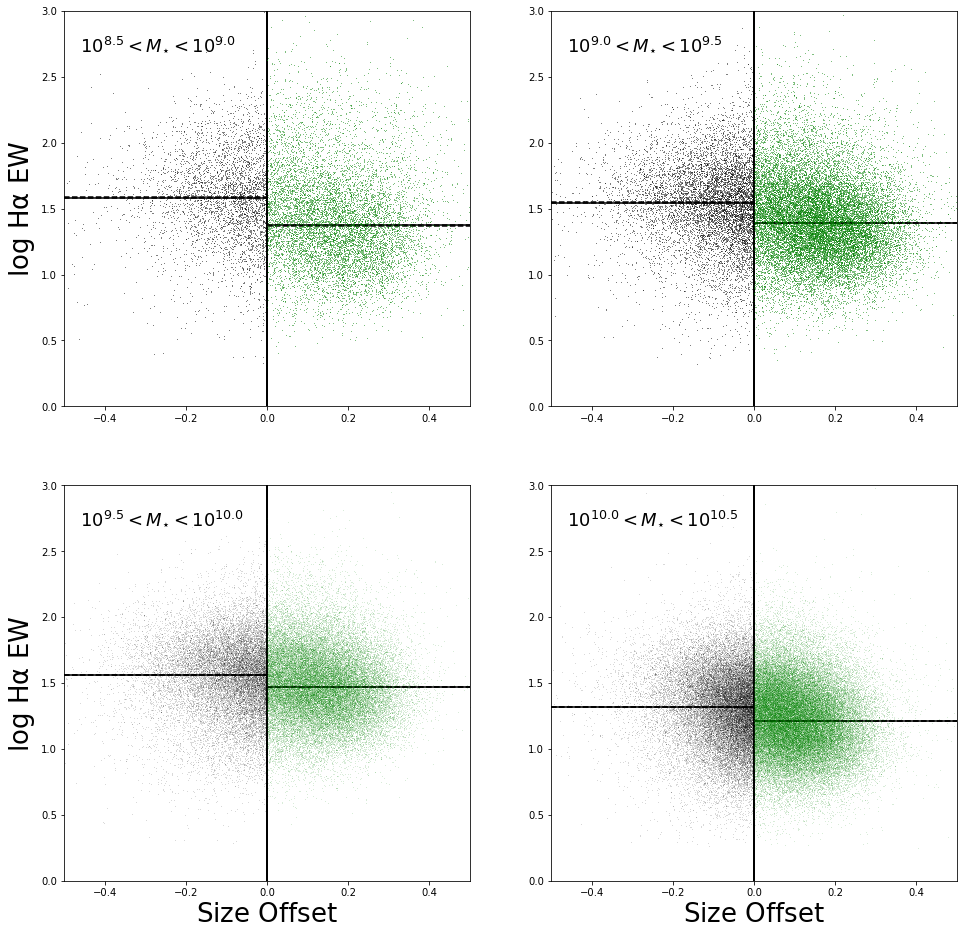
\includegraphics[width=1.5 \columnwidth]{ha_ew_2x2.png}
%	\caption{$H\alpha$ rest frame equivalent width plotted against galaxy size offset size offset in four different mass bins. The data are anticorrelated at all masses, but show stronger anticorrelation at low masses. Black and green points represent smaller-than-average and larger-than-average galaxies, respectively. Horizontal lines indicate median equivalent widths for the small and large portions of each bin. }
%	\label{fig:HA_ew}
	
%\end{figure*}
%%%%%%%%%%%%%%%%%%%%%%%%%%%%%%%%%%%%%%%%%%%%%%%%%%%%%%%%%%%%%% 

%%%%%%%%%%%%%%%%%%%%%%%%%%%%%%%%%%%%%%%%%%%%%%%%%%%%%%%%%%%%%%
%\begin{figure}
%	\centering
%	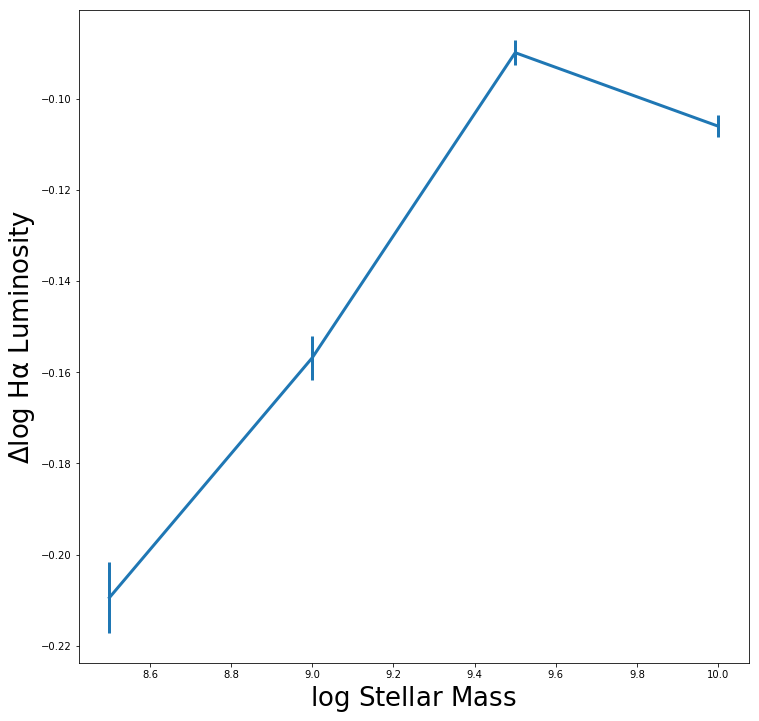
\includegraphics[width= \columnwidth]{ratios_ha_ew.png}
%	\caption{Change in median rest-frame $H\alpha$ equivalent width between the objects with size offset greater than zero and objects with size offset less than zero plotted against stellar mass.}
%	\label{fig:HA_ew_mass}
	
%\end{figure}
%%%%%%%%%%%%%%%%%%%%%%%%%%%%%%%%%%%%%%%%%%%%%%%%%%%%%%%%%%%%%% 


%%%%%%%%%%%%%%%%%%%%%%%%%%%%%%%%%%%%%%%%%%%%%%%%%%%%%%%%%%%%%%
\begin{figure*}
	\centering
	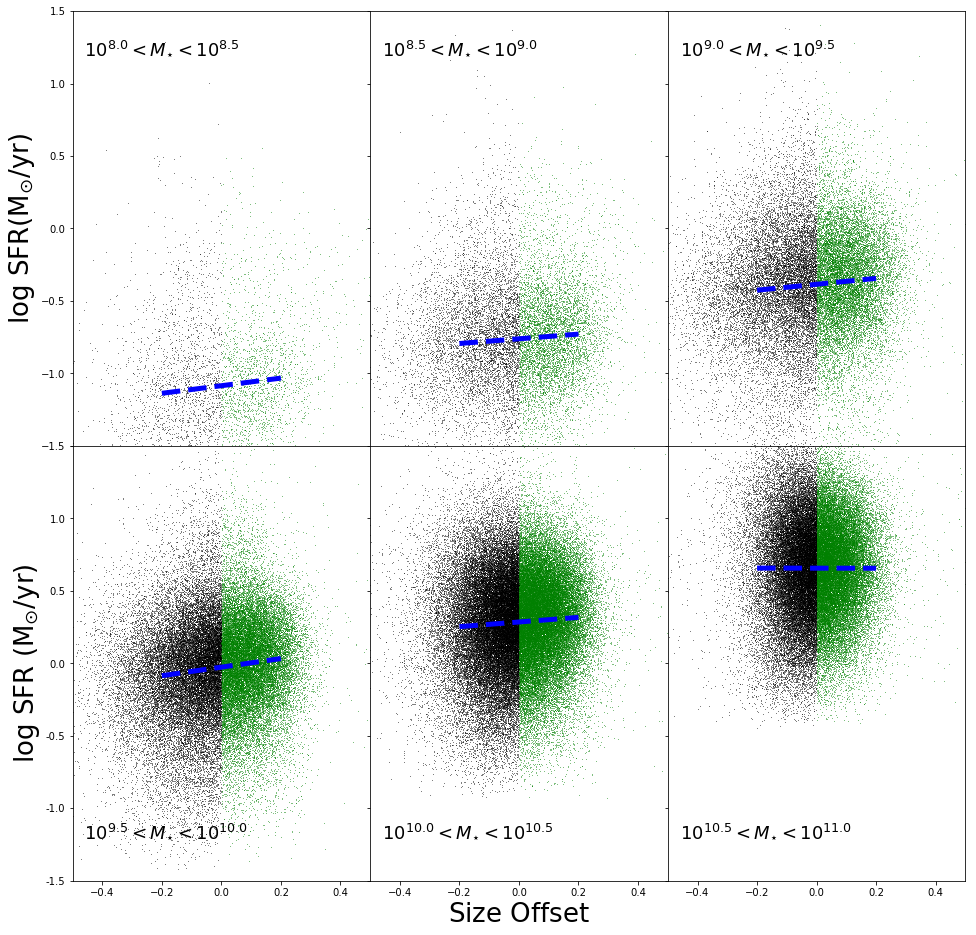
\includegraphics[width=1.5 \columnwidth]{ha_lum_2x2_2A.png}
	\caption{Star formation rate plotted against size offset for galaxies in four mass bins. The data transition from a nearly flat relation at small masses to a slight correlation at larger masses. Black and green points represent smaller-than-average and larger-than-average galaxies, respectively. Blue dashed line is a linear fit to the data.}
     \label{fig:sfr}

\end{figure*}
%%%%%%%%%%%%%%%%%%%%%%%%%%%%%%%%%%%%%%%%%%%%%%%%%%%%%%%%%%%%%% 

%%%%%%%%%%%%%%%%%%%%%%%%%%%%%%%%%%%%%%%%%%%%%%%%%%%%%%%%%%%%%%
\begin{figure}
	\centering
	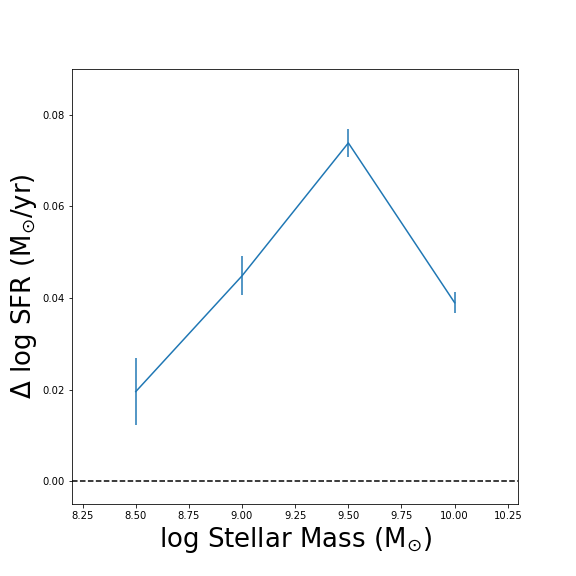
\includegraphics[width= \columnwidth]{mass_delta_sfr.png}
	\caption{Change in median $H_{\alpha|}$ luminonsity between the objects with size offset greater than zero and objects with size offset less than zero plotted against stellar mass.}
	\label{fig:HA_lum_mass}
	
\end{figure}
%%%%%%%%%%%%%%%%%%%%%%%%%%%%%%%%%%%%%%%%%%%%%%%%%%%%%%%%%%%%%% 


%%%%%%%%%%%%%%%%%%%%%%%%%%%%%%%%%%%%%%%%%%%%%%%%%%%%%%%%%%%%%%
\begin{figure*}
	\centering
	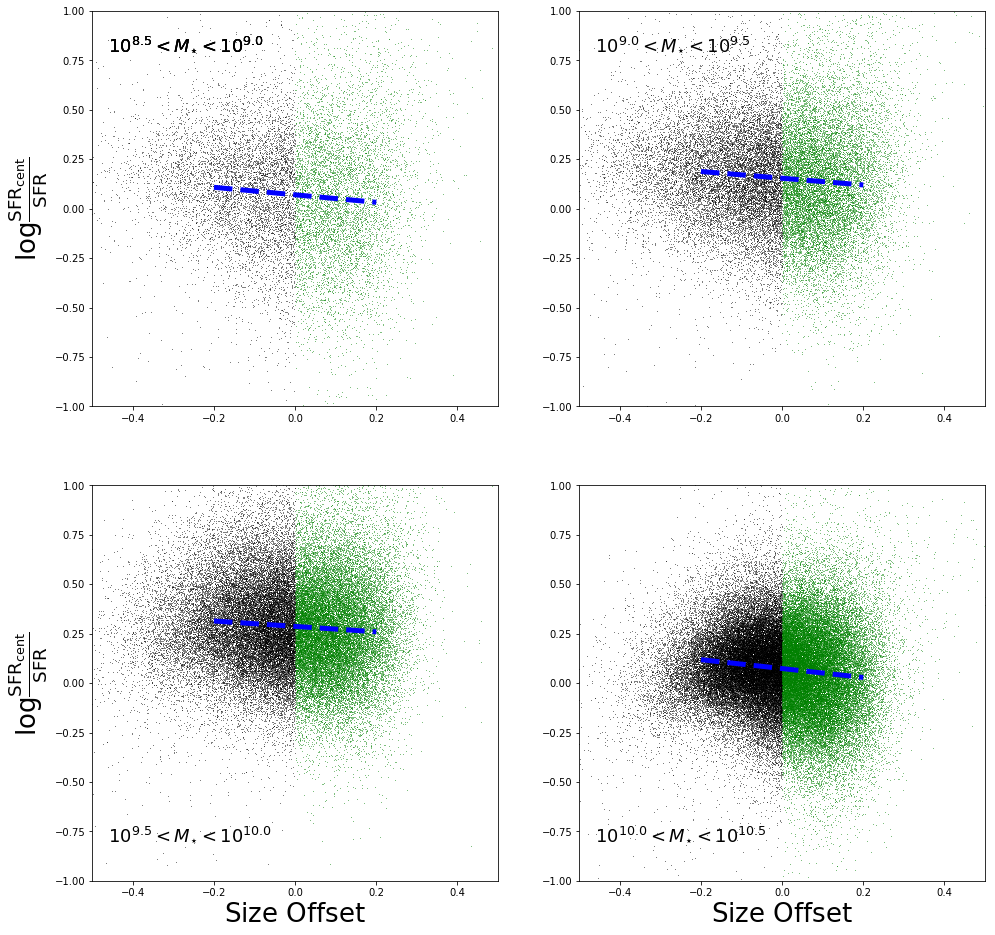
\includegraphics[width=1.5 \columnwidth]{ha_lum_2x2_excess.png}
	\caption{Star formation rate plotted against size offset for galaxies in four mass bins. The data transition from a nearly flat relation at small masses to a slight correlation at larger masses. Black and green points represent smaller-than-average and larger-than-average galaxies, respectively. Blue dashed line is a linear fit to the data.}
	\label{fig:conc1}
	
\end{figure*}
%%%%%%%%%%%%%%%%%%%%%%%%%%%%%%%%%%%%%%%%%%%%%%%%%%%%%%%%%%%%%% 

%%%%%%%%%%%%%%%%%%%%%%%%%%%%%%%%%%%%%%%%%%%%%%%%%%%%%%%%%%%%%%
\begin{figure}
	\centering
	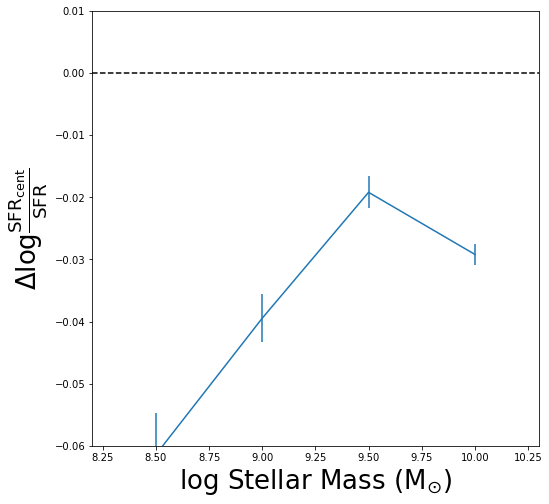
\includegraphics[width= \columnwidth]{mass_delta_cent.png}
	\caption{Change in median $H_{\alpha|}$ luminonsity between the objects with size offset greater than zero and objects with size offset less than zero plotted against stellar mass.}
	\label{fig:conc2}
	
\end{figure}
%%%%%%%%%%%%%%%%%%%%%%%%%%%%%%%%%%%%%%%%%%%%%%%%%%%%%%%%%%%%%% 



%%%%%%%%%%%%%%%%%%%%%%%%%%%%%%%%%%%%%%%%%%%%%%%%%%%%%%%%%%%%%%
\begin{figure*}
	\centering
	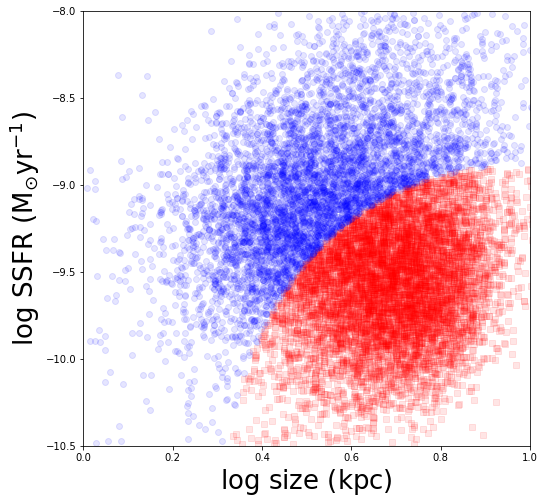
\includegraphics[width=1. \columnwidth]{GMM.png}
	\caption{Black line divides the lowest mass sample into actively and passively star-forming galaxies as derived from a Gaussian mixture model. Approximately 57\% of the sample is in the passive regime, while 43\% is in the active regime.}
     \label{fig:HA_duty}

\end{figure*}
%%%%%%%%%%%%%%%%%%%%%%%%%%%%%%%%%%%%%%%%%%%%%%%%%%%%%%%%%%%%%% 


%\subsection{Radial dependencies}

%Here we present the radial profiles in $H_{\alpha}$ luminosity for galaxies in our sample. In addition to each galaxy's total $H_{\alpha}$ luminosity, we can probe the properties at the physical radius corresponding to the radius of the fiber. Then, by binning in physical radius, we can construct the average $H_{\alpha}$ profile for galaxies in each mass bin.

%Figure \ref{fig:grad_lum} shows this average $H\alpha$ luminosity profile among galaxies across the four mass bins. At small radii (below $\rm \log R =0.6$), the galaxies obey the same power law relationship across all four mass bins. Above that radius, the low mass points fall off of this power law relation while the high mass points continue along the power law. Physically, this means that low mass galaxies have very little $H\alpha$ at larger radii, while high mass galaxies have similar amounts at all radii.


%%%%%%%%%%%%%%%%%%%%%%%%%%%%%%%%%%%%%%%%%%%%%%%%%%%%%%%%%%%%%%
%\begin{figure*}
%	\centering
%	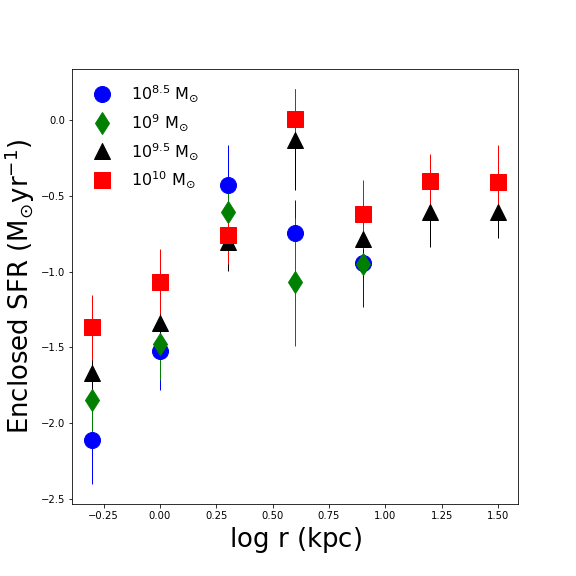
\includegraphics[width= \columnwidth]{gradients_HA_SFR.png}
%	\caption{Average SFR profile for galaxies in four different mass bins. Each individual galaxy contributes twice to the plot: once at the fiber radius, and once at the galaxy radius. Galaxies contribute non-uniformly to the plot, resulting in non-monotonically increasing profiles}
%     \label{fig:grad_lum}

%\end{figure*}
%%%%%%%%%%%%%%%%%%%%%%%%%%%%%%%%%%%%%%%%%%%%%%%%%%%%%%%%%%%%%% 

\section{Discussion}
\label{(sec:discuss)}
%\subsection{Radial Dependencies}

%In Section \ref{sec:obs}, we describe our method for correcting spectroscopic measurements for regions of the galaxy that lie outside the SDSS fiber. To summarize, we define $\Psi$ as the fraction of the galaxy that lies within the fiber, and assume the correction factor is a power law in $\Psi$, with the power law index determined empirically.

%Because we can correct for fiber effects we can use both the fiber and corrected measurement to probe the galaxy at two radii, the fiber radius and size of the galaxy itself. This allows us to plot radial profiles for $H\alpha$ luminosity. In high mass galaxies, the profile is consistent with a single power law at all radii, whereas in galaxies below $10^{9.5} \rm M_{\odot}$ in stellar mass, the profile resembles a broken power law. The power law slope is consistent with the high mass slope at small radii, but at intermediate radii it flattens out, consistent with no $H\alpha$ emission at larger radii. Although we have limited spatial resolution, we can estimate that the transition radius occurs at $3-4$ kpc.

%The presence of $H\alpha$ purely at the center of dwarf galaxies is significant evidence against the idea that they are currently forming stars in their outskirts. Although it is tempting to conclude that dwarf galaxies only ever form stars in their interiors, we are only looking at low-redshift dwarfs. Our observations do not rule out the possibility that dwarfs may experience extended star formation early in their histories and centrally-concentrated later in their histories. However, detailed studies of local dwarfs' star formation histories show a wide range of formation times, implying that our sample contains dwarf galaxies in all phases of their star formation history. If dwarf galaxies formed stars in their outer regions at any points during their history, we would expect to see some extended star formation reflected in the radial profiles. This is not observed; however, it is possible that extended star formation in dwarf galaxies took place at an earlier stage in the Universe's history. Similar observations at higher redshift would rule out this possibility.

%%%%%%%%%%%%%%%%%%%%%%%%%%%%%%%%%%%%%%%%%%%%%%%%%%%%%%%%%%%%%%
%\begin{figure*}
%	\centering
%	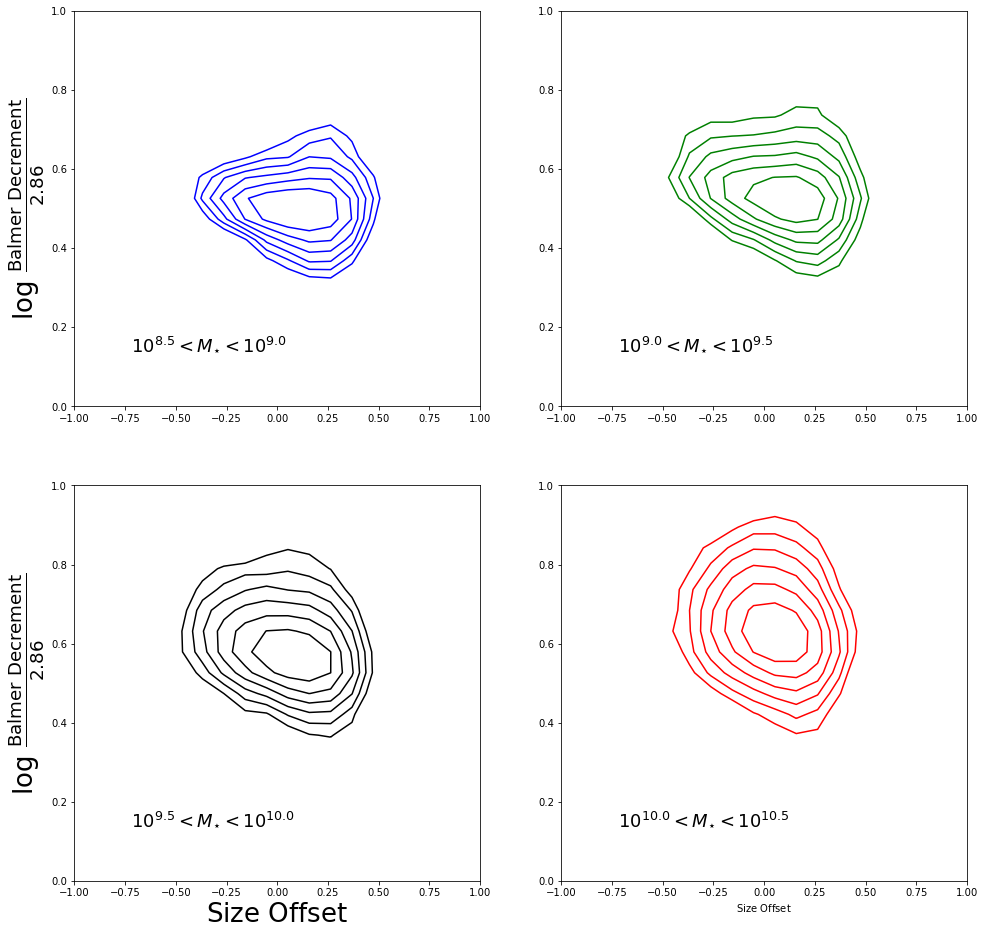
\includegraphics[width=1.5 \columnwidth]{Balmer_dec.png}
%	\caption{Balmer decrement vs. size offset for dwarf galaxies. Galaxies show progressively more reddening at higher masses and at smaller sizes. This demonstrates that our results do not depend on excess reddening at large sizes, and the effects we see are strongest when reddening is weakest (i.e. at low mass).}
 %    \label{fig:bdvsize}

%\end{figure*}
%%%%%%%%%%%%%%%%%%%%%%%%%%%%%%%%%%%%%%%%%%%%%%%%%%%%%%%%%%%%%% 


\subsection{Galaxy Size}

An important prediction of the ``breathing'' model of feedback regulation in dwarf galaxies is that star formation rate is anticorrelated with galaxy size. In the model, stars are formed in the galactic center. The young stars then produce supernova feedback, which blows out the reservoir of gas from which the stars were formed, dampening star formation. As a result, galaxies are actively forming stars when they are at their smallest. During the subsequent blowout phase the galaxy will be more diffuse and, if the galactic wind drives radial transport, the galaxy will have a larger effective radius \citep{EB17}. 

Our results give compelling evidence for this prediction below $10^{9.5} M_{\odot}$, suggesting that dwarf galaxies form stars in a ``breathing" mode. Importantly, this result combined with the lack of $H\alpha$ seen in galactic outskirts of dwarfs suggests that the energy produced during episodes of star formation couples to the stars in the galactic center and drives stellar radial transport.

There are, however, potential alternate explanations for the observed anti-correlation between H$\alpha$ emission and galaxy size. We will briefly discuss these. Firstly, we will consider the possibility that galaxies at different sizes do form stars at the same rate, but different amounts of $H\alpha$ emission escape the galaxy. This could be due to variations in the initial mass function (IMF), which sets the rates at which stars of different masses form. A top-heavy IMF, where more massive stars are formed relatively more frequently, would result in more ionizing radiation being formed per unit star formation. Our results could potentially be explained by smaller galaxies having more top-heavy IMFs. Whether or not the IMF varies between galaxies, or within galaxies, is an area of active research, with most results being consistent with a universal IMF \citep[e.g.,][]{Lee09,Bastian10}. 

An alternate possibility is that galaxies form stars at the same rate and as described by the same IMF at the same mass, but dust obscures star formation in such a way as to create a trend where there would otherwise be none. However, previous studies have shown that dust reddening increases with increasing stellar mass \citep{Garn10}, leaving it unlikely to drive an effect seen primarily at dwarf masses. We see a similar result in our data, with Balmer decrement increasing with increasing galaxy mass. Thus we conclude that dust extinction is unlikely to be the driver of the effects we see.

\subsection{Duty Cycle and Energetics}

In Section \ref{sec:results}, we divide the galaxies in our lowest mass bin into actively and passively star forming subcategories via a Gaussian process decomposition. We draw an important distinction between \textit{passively star forming} galaxies, which still show signs of ongoing star formation, and \textit{passive galaxies}, which no longer are forming stars. The latter are outside the scope of this paper, having been eliminated from our sample by our $H_{\alpha}$ equivalent width cut. We define the duty cycle of this population to be the fraction of time a galaxy spends in its active phase, as estimated by the fraction of galaxies observed to be in the active phase, and measure this value to be 0.42; i.e., dwarf galaxies spend roughly forty percent of their lifespan in a phase where they are actively forming stars and the other sixty percent not in this phase. Due to the increased size of the galaxy during the passively star forming phase, we will interpret this to be the phase where the galaxy is undergoing stellar feedback-driven blowouts. There are several different interpretations for this measured duty cycle that we now discuss.

Firstly, we will examine this number under the view that the instantaneous star formation rate in dwarf galaxies at a particular time is a stochastic sampling of an underlying probability distribution of star formation rates. Of course, this view is only sensible as an approximation; nevertheless, there are benefits to thinking of star formation in this way, particularly as it pertains to generating analytic and semi-analytic models \citep{Kelson16}. 

Under this probabilistic interpretation, a galaxy's star formation rate represents a sampling of an underlying star formation rate probability distribution function. Our result suggest that the probability of galaxies being in the quiescent state is twice as high as the galaxies in the active state. We draw a distinction between this quiescent phase and final quenching, when a galaxy becomes ``red and dead." This final quenching phase is likely not a result of stochastic sampling of an underlying pdf, but rather the result of physical processes that bring the galaxy out of the ``breathing'' mode and into the ``red and dead'' mode. In particular, galaxies at these masses are predominantly quenched through environmental means \citep{Kauffmann03, geha12}.

Physically, we can interpret duty cycle in terms of the times a galaxy spends in each phase in order to explore the physicals scalings and energetics involved. As an example, we use the test case of a $10^9 M_{\odot}$ galaxy of radius 5 kpc. Assuming that the blowout moves with the speed $v_{wind}$, the total time it takes to reach the edge of the galaxy is $\frac{R}{v_{wind}}$. If the material takes the same amount of time to fall back onto the center as to reach the galactic outskirts, then the total time spent in the passive phase is twice this time. Using the duty cycle implied by Figure \ref{fig:HA_duty}, we can conclude empirically that the time spent in the active phase during a single burst is $$t_{active} = \frac{4 \times R}{5 \times v_{wind}} = 13.0 Myr \times \frac{R}{5 kpc}\times \frac{300 km/s}{v_{wind}}  $$, consistent with the timescales put forward by \cite{EB17}. Multiplying this value by the star formation rate of objects in the active phase gives us the total number of stars formed in one cycle:
$$\Delta M_{\star} = 6.4 \times 10^5 M_{\odot} \times \frac{SFR}{0.062 M_{\odot}/yr} \times \frac{t_{active}}{13.0 Myr}$$.

The IMF allows us to connect the amount of star formation in a burst to the strength of the supernova feedback produced by that burst. Under a Kroupa IMF \citep{Kroupa02}, we expect one Type II supernova for every 100 solar masses in stars formed, meaning that a single burst in a dwarf galaxy produces some $8 \times 10^3$ Type II supernova. Given that the average energy output of a Type II supernova is $10^{51}$ erg, the total energy output during a single burst is $10^{55}$ erg. In order to produce $10^9 M_{\odot}$ of stellar mass, the galaxy must have gone through $10^3$ cycles, thereby producing $10^{58}$ erg of supernova energy in the process. The energetic argument presented in the above paragraph is true independent of whether the stars are formed constantly or in bursts. However, as several authors have argued \citep{Governato12,GK13}, the ``bursty'' mode of star formation can produce a positive feedback cycle, where the the efficiency of subsequent bursts increases from the initial burst \cite[see][]{Pontzen12,Governato12}. 

%To further examine how energetics of a ``bursty" galaxy can drive core formation, let us consider two spherically symmetric dark matter halos of total mass $10^9 \rm M_{\odot}$ within 10 Mpc, both with core radii of $r_0 = 400$ pc, both with total radii of $r_{max} = 100$ kpc and both with double power law density profiles: $$\rho(r) = \frac{\rho_0}{(r/r_0)^a(1+r/r_0)^b}$$.
%We will consider the first halo to have  an NFW profile (a=1,b=2) \cite{NFW}, while the second has a flat inner profile (a=0,b=3). We can integrate the expression $$U = -G\int_{0}^{r_{max}} \frac{M(<r) \rho(r) dV}{r}$$ to compute the gravitational binding energy for each halo. Carrying this integral out, we find a binding energy of $-5.04 \times 10^{56}$ erg for the NFW halo and $-3.61\times 10^{56})$ erg for the cored halo. Thus, we must input at least $1.42 \times 10^{56}$ erg in order to go from an NFW halo to a cored halo at halo mass $10^{9} \rm M_{\odot}$. 

%We turn now to examine supernova as the source of this energy. We may write the amount of energy that each supernova contributes to the system as $\epsilon \chi E_{SN}$, where $\epsilon$ is the ``natural" coupling efficiency between a single supernova and the surrounding dark matter, $\chi$ is the boost in efficiency due to positive feedback from the previous bursts, and $E_{SN}$ is the amount of energy released in a single supernova. Thus, the total energy deposited in the halo is $$E = \sum_{i = 1}^{n_{SN}} \epsilon \chi_i E_{SN} = \epsilon <\chi> n_{SN} E_{SN}$$. We can use the previously-discussed values for the energy released by supernova over a dwarf galaxies and for the energy required to produce a core to arrive at $\epsilon <\chi> = 0.014$; however, there is much physics hiding in the $\chi_{i}s$. For example, the star formation histories of more-massive galaxies are less bursty \citep{Guo16} than those of dwarf galaxies, so the coupling between the supernova and the dark matter is likely smaller, preventing core formation. Examining dwarf galaxies at higher redshift will shed further light on the evolution of their density profiles and how density cores are produced over cosmic time.

\subsection{Comparisons to Simulations}

Hydrodynamical simulations whereby galaxy growth is regulated through burst-driven radial transport make a number of specific, testable predictions of galaxy observables. We divide our discussion of these predictions into two sections: predictions concerning galaxy dynamics, which we do not address but is addressed by \cite{Cicone16}, and predictions concerning galaxy structure, which is the primary concern of this work.

The burst-driven transport model of galaxy self-regulation requires that feedback not only couple to the gas in a galaxy, but also to the stellar component. As a result, the stars are kinematically heated, resulting in an increased line of sight velocity dispersion. \cite{El-Badry17} makes this prediction explicit, demonstrating a correlation between $\sigma_{LOS}$ and specific star formation rate for star particles in the final 40 snapshots of one simulated dwarf galaxy halo. Under the assumption that the evolution of this single halo is an ergodic process, this supplies a prediction for the population of dwarf galaxies at low redshift.

These predictions are borne out by the analysis of \cite{Cicone16}, which uses stacked SDSS spectra to examine the profiles of nebular emission lines and stellar absorption lines, constraining the dynamics of galactic gas and stars respectively. They find that, for dwarf galaxies, the width of stellar absorption lines increases with increasing specific star formation rate, consistent with the predictions of \cite{El-Badry17}. Furthermore, they find that this trend disappears above stellar masses of $10^{9.5} M_{\odot}$, consistent with the prediction that burst-driven transport only operates at dwarf mass scales.

We can also compare the trends with size that we have explored in this work to predictions from hydrodynamical simulations. In Figure \ref{fig:predict}, we over plot the final 40 snapshots from a dwarf galaxy in the FIRE simulation with galaxies from our lowest-mass bin ($10^{8.5}-10^{9.0} M_{\odot}$) in specific star formation rate/size space. Again, we emphasize that since the simulated galaxies evolve in this space, the points traced by the galaxy in the simulation make a prediction for galaxies sampled in the real Universe. We see agreement between the predictions made by the simulation and our observed relationship between specific star formation rate and size. There is significantly more scatter in the observed relation than the simulation results, which is a natural result of comparing an ensemble of galaxies with a single simulated object, but the overall agreement between simulations and data is striking. Taken together, these two observational confirmations of simulation predictions provide strong evidence that burst-driven radial transport is occurring in dwarf galaxies.



%%%%%%%%%%%%%%%%%%%%%%%%%%%%%%%%%%%%%%%%%%%%%%%%%%%%%%%%%%%%%%
\begin{figure*}
	\centering
	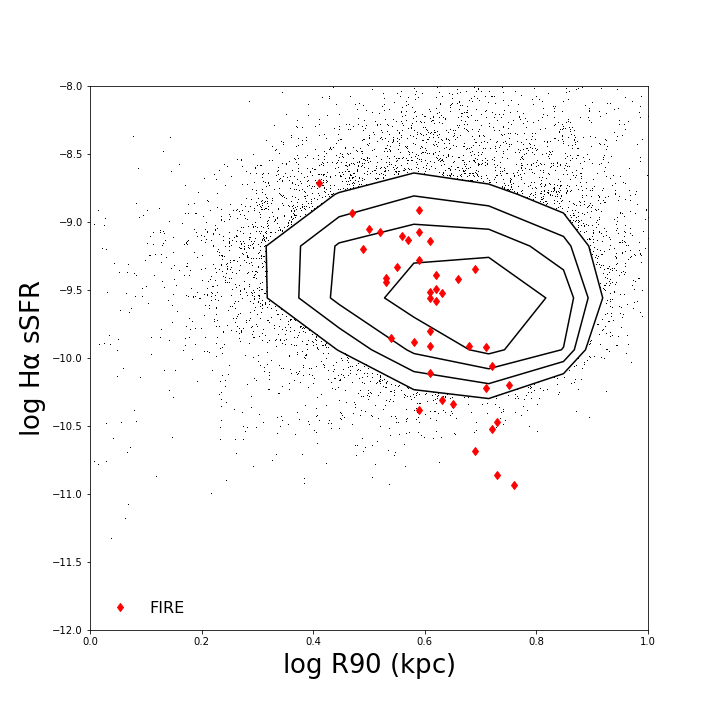
\includegraphics[width=1.5 \columnwidth]{111_dwarf_8_5_size_SF_r.png}
	\caption{Star formation rate plotted against size for galaxies in our lowest mass bin. Overplotted are points from the last 40 snapshots of a dwarf galaxy in the FIRE simulation that is undergoing self-regulation via burst-driven radial transport. The data is in excellent agreement with the predictions from the simulations}
	\label{fig:predict}
	
\end{figure*}
%%%%%%%%%%%%%%%%%%%%%%%%%%%%%%%%%%%%%%%%%%%%%%%%%%%%%%%%%%%%%% 

\section{Conclusion}

Our study primarily examines the relationship between the physical size of a galaxy and it's star formation properties. We show the following,

\begin{itemize}
\item Dwarf galaxies with smaller size tend to have higher levels of $H\alpha$ emission. Dwarf galaxies of larger size have lower levels of $H\alpha$ emission. This trend goes away in more massive galaxies. 

\item $H\alpha$ surface density is consistent with a power law with respect to radius in the inner regions of galaxies at all masses, however in dwarf galaxies, the outer regions have $H\alpha$ emission consistent with zero.

\item Taken together, these results paint a picture in which dwarf galaxies experience cycles of star formation, where dense star formation in the central regions drives blowouts that self-regulate galaxy growth. Furthermore, our results are in strong agreement with simulations that exhibit such blowouts. The energy of the blowouts couples to the stars, leading to dwarf galaxies in their blowout phase being larger on the sky in the $r$ band.

\end{itemize}

\bibliographystyle{ApJ}
\bibliography{biblio}

%\appendix{Comparison to color-based aperture corrections}

%Here we compare our aperture correction method to one similar to that of \cite{Brinchmann04}. In order to correct for the size of the SDSS fiber, the authors developed a methodology whereby a spectroscopic measurement (e.g. star formation rate) was associated with the fiber $gri$ colors of the galaxy, the the properties of the galaxy outside of the fiber were inferred from the gri colors of the portion of the galaxy located outside of the fiber. Here, we adopt a similar methodology for the purposes of comparison. 

%%We adopt a simple, yet effective relation to estimate $H\alpha$ equivalent width from galaxy color:

%%$$\rm log EW_{H\alpha} = 2-%%2\times(\textit{g-r}) $$

%%

%We first make use of the fiber g-r and r-i colors to estimate to estimate the measured fiber equivalent width. We divide the sample in half, and use the two colors as features in decision-tree regression algorithm fit to fiber $H\alpha$ equivalent widths. We then use the algorithm to predict the fiber $H\alpha$ equivalent width in the unused half of the sample. The agreement between the prediction derived from the colors and the spectroscopic measurement is seen in Figure \ref{fig:ccheck}. Then, we estimate the total $H\alpha$ equivalent width from the galaxies' total colors. The red contours in Figure \ref{fig:ccheck} demonstrate the agreement between the equivalent width estimated in this way and the equivalent width determined from the fiber corrections described in \ref{sec:fibercor}.

%Below $10^{9.5}$ solar masses, we see the agreement between the two methodologies break down. Predictions of total galaxy $H\alpha$ equivalent widths based on fiber color will tend to be overestimates, particularly in low equivalent width systems. This observation  in line with what \cite{Salim07} argued; the relation between color and SSFR established in star forming galaxies breaks down in galaxies without $H\alpha$. We point out that this also extends to regions of galaxies that do not emit $H\alpha$, which impacts fiber corrections even within star forming galaxies.

%%%%%%%%%%%%%%%%%%%%%%%%%%%%%%%%%%%%%%%%%%%%%%%%%%%%%%%%%%%%%%
%\begin{figure*}
%	\centering
%	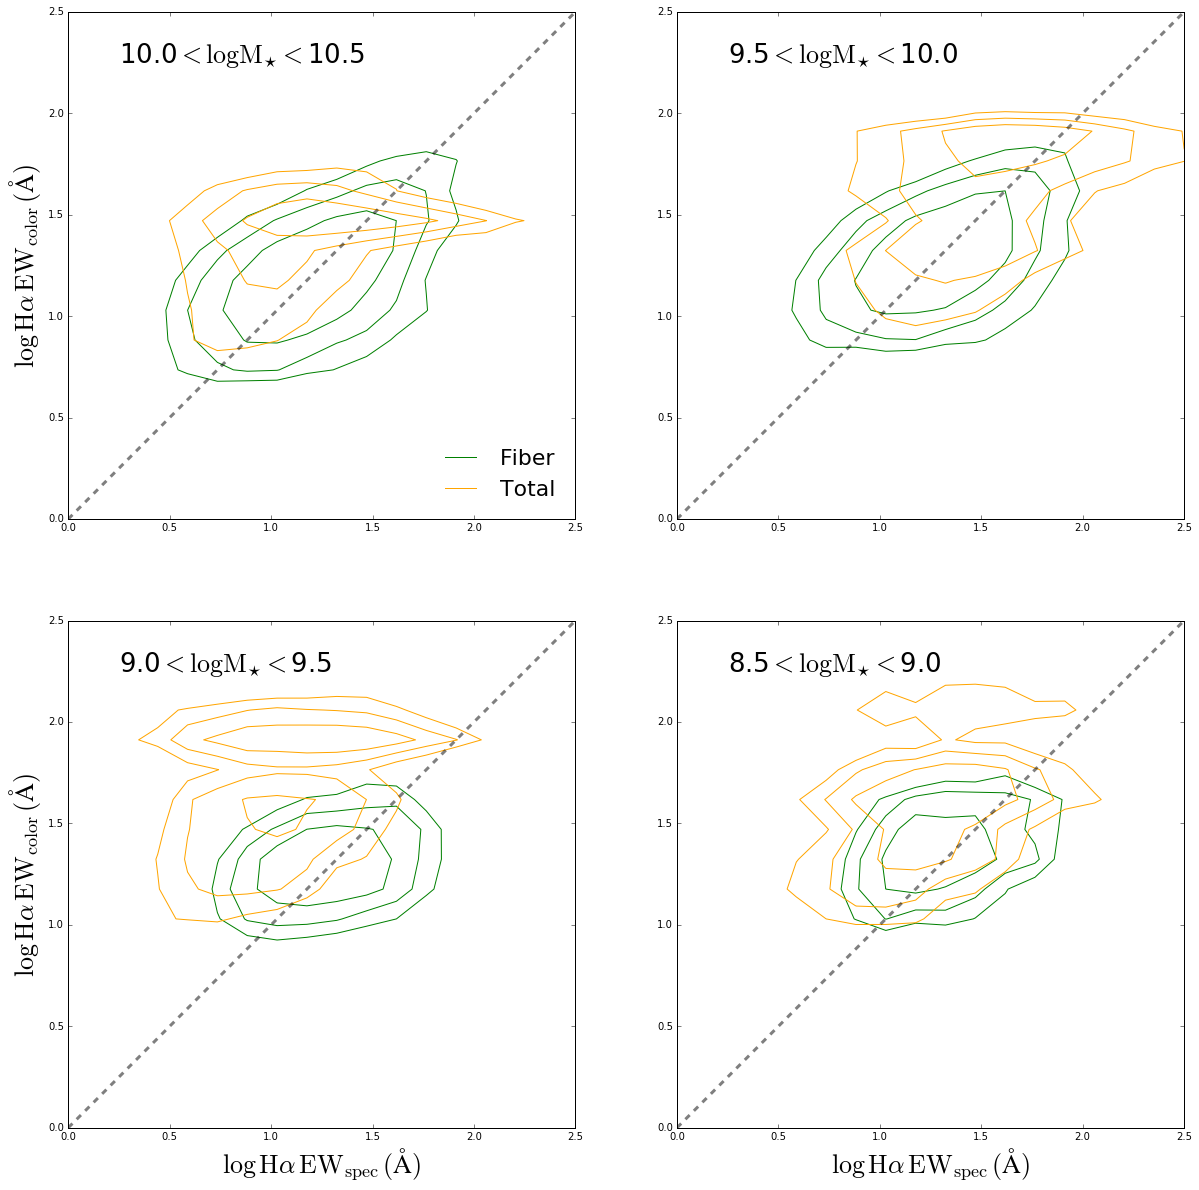
\includegraphics[width= \columnwidth]{HA_EW_compare.png}
%	\caption{Comparison between photometrically-derived and spectroscopically-derived $\rm H\alpha$ equivalent widths for galaxies in our science sample (see text for details). Blue contours are the $H\alpha$ within the fiber and red contours are total $H\alpha$. At low masses, the photometrically derived total $H\alpha$ is overestimated.}
%     \label{fig:ccheck}

%\end{figure*}
%%%%%%%%%%%%%%%%%%%%%%%%%%%%%%%%%%%%%%%%%%%%%%%%%%%%%%%%%%%%%% 

\end{document}

%%
%% End of file `sample.tex'.
